\section{Final results and conditional ablation study}\label{sec:results}

\subsection{Final four-model results}
The final release reports two quantitative tables because its two generation modes answer different questions. Conditional endpoints are sampled for 40 ID and 40 compositional-OOD structured prompts, with five seeds per prompt (400 authenticated images per endpoint), then scored by the frozen CartoonSet100k dual-view evaluator. Unconditional endpoints are 400 marginal samples with no requested attributes. The sources, evaluator, pool, sampler, and endpoint digests are given in \cref{app:provenance}.

\begin{table*}[htbp]
\centering\small
\caption{Final conditional public endpoints under the authenticated supplementary structured-prompt application. KID/FID are Common-32; LPIPS is native-resolution, within-prompt and across seed; MAA/EAM/MacroPSR are OOD evaluator measures. The 80-prompt, five-seed panel is reused supplementary evidence, not a newly independent sealed holdout.}\label{tab:conditional-final}
\begin{tabular}{lrrrrrrr}
\toprule
Endpoint & KID & FID$^{\dagger}$ & LPIPS ID/OOD & OOD MAA & EAM & MacroPSR \\
\midrule
H7 conditional, native32, EMA-40k & .010000 & 59.430 & .028743/.026561 & .965 & .860 & .895 \\
V2-A conditional, native64, EMA-60k & .016694$^{*}$ & 65.007$^{*}$ & .095535/.089085$^{*}$ & .980 & .920 & .960 \\
\bottomrule
\end{tabular}
\par\smallskip\footnotesize $^{*}$Native64 images use a provenance-recorded 64-to-32 LANCZOS route for Common-32 quality; LPIPS remains native64 and is not a cross-resolution diversity rank. $^{\dagger}$FID is an exploratory finite-sample plug-in estimate. Source: STEP~9B/10 records in \cref{app:provenance}.
\end{table*}

\begin{table*}[htbp]
\centering\small
\caption{Final unconditional public endpoints from the completed STEP~13 marginal-sampling protocol. Each row uses 400 generated samples, Common-32 KID/FID against the 808-image real pool, and 200 deterministic disjoint marginal LPIPS pairs. MAA, EAM, and MacroPSR are not defined because no structured request is supplied.}\label{tab:unconditional-final}
\begin{tabular}{lrrrrrr}
\toprule
Endpoint & KID & FID$^{\dagger}$ & marginal LPIPS & parameters & latency (s/image) & peak bytes \\
\midrule
V1 unconditional, native32, EMA-40k & .008134 & 41.547 & .088892 & 4\,595\,779 & 6.150 & 30\,732\,288 \\
V2-A unconditional, native64, EMA-60k & .009724$^{*}$ & 47.215$^{*}$ & .234633$^{*}$ & 5\,077\,123 & 8.013 & 37\,800\,960 \\
\bottomrule
\end{tabular}
\par\smallskip\footnotesize $^{*}$Common-32 derives RGB64 outputs by LANCZOS downsampling; native64 LPIPS is not an absolute diversity ranking against native32. $^{\dagger}$FID is exploratory. Latency/memory are endpoint-specific RTX 4060 Laptop GPU measurements with the recorded 1,000-step ancestral DDPM contract. Source: completed STEP~13 summary and endpoint metrics in \cref{app:provenance}.
\end{table*}

The shared Common-32 calculation does not make conditional and unconditional samples a directly comparable experimental distribution: the former is driven by structured ID/OOD prompts and the latter by a marginal sampling plan. Conditional LPIPS contains ten unordered within-prompt pairs per prompt, whereas unconditional LPIPS pairs sorted marginal samples at ranks $i$ and $i+200$. Thus neither LPIPS column supports a cross-mode comparison, and conditional-versus-unconditional differences at a resolution are descriptive rather than causal effects of conditioning.

\subsection{Conditional ablation study}
The CA16 and native64 decisions were made from historical development records, not from the later standardized values below. The historical native32 evaluator, subsequent evaluator development, frozen dual-view evaluator, sealed registry, and Common-32/LPIPS contracts have distinct roles; their provenance and non-interchangeability are audited in \repoPath{docs/release/HISTORICAL_EVALUATION_AND_DECISION_AUDIT.md}. No unauthenticated historical glasses-accuracy value is used as quantitative evidence.

\begin{table*}[htbp]
\centering\small
\caption{Five authentic conditional endpoints under the same supplementary measurement family. KID/FID are Common-32; LPIPS is within-prompt, across-seed and native-resolution. The table preserves the ablation chain, not a fifth-to-ninth public model list.}\label{tab:conditional-chain}
\begin{tabular}{lrrrrrrrr}
\toprule
Endpoint & px & updates & KID & FID & LPIPS ID/OOD & OOD MAA & EAM & MacroPSR\\
\midrule
V1 conditional CA8 & 32 & 20k & .039188 & 96.519 & .037824/.034455 & .2950 & .000 & .000\\
H7 CA8+CA16 & 32 & 20k & .036479 & 93.531 & .035748/.033109 & .4013 & .010 & .045\\
H7 CA8+CA16 & 32 & 40k & .010000 & 59.430 & .028743/.026561 & .965 & .860 & .895\\
V2-A CA8+CA16 & 64 & 40k & .027882$^*$ & 75.379$^*$ & .108116/.103626$^*$ & .645 & .055 & .385\\
V2-A CA8+CA16 & 64 & 60k & .016694$^*$ & 65.007$^*$ & .095535/.089085$^*$ & .980 & .920 & .960\\
\bottomrule
\end{tabular}
\par\smallskip\footnotesize $^*$For V2-A, Common-32 is a 64-to-32 LANCZOS-derived quality route and LPIPS is native64; these are not native-detail or cross-resolution rankings. STEP~9B/10 are supplementary reuse of an existing panel, not a new independent holdout.
\end{table*}

The four primary comparisons are: (A) V1 conditional CA8-20k to H7-20k, associated with CA16 but confounded by independent trajectories and +25\,152 parameters; (B) H7-20k to H7-40k, an authenticated exact-state continuation; (C) H7-40k to V2-A-40k, a joint change in resolution, architecture, and preprocessing; and (D) V2-A-40k to V2-A-60k, an authenticated exact-state continuation. The CA8-40k versus H7-40k native32 comparison is retained as additional evidence: H7 exceeds CA8 by .015 OOD MAA and .060 EAM, with paired 95\% bootstrap intervals $[.0025,.02875]$ and $[.010,.115]$; it still estimates the complete CA16 intervention rather than attention placement alone. None of these point-estimate differences is a general significance claim.

\begin{figure}[htbp]
\centering
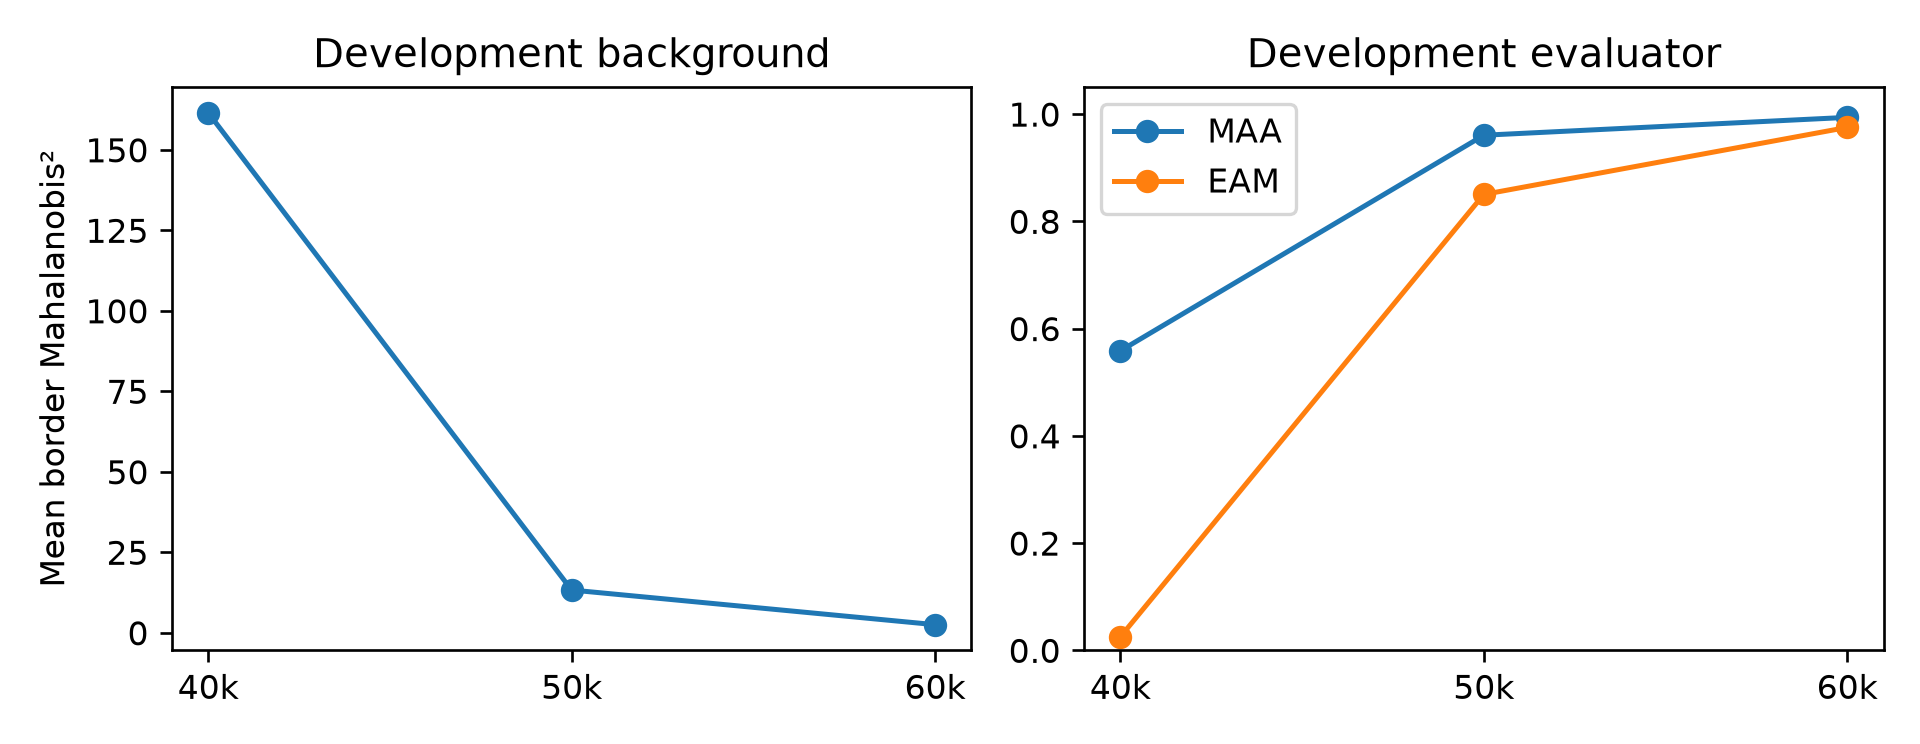
\includegraphics[width=.92\linewidth]{figures/figure_step9a_development.png}
\caption{Development-only matched native64 40k--50k--60k trajectory on 120 non-protected cases. Border Mahalanobis$^2$ is a background diagnostic; evaluator MAA/EAM are descriptive development measurements, not official pair-specific MacroPSR. Source: STEP~9A development asset preserved by STEP~9B.}\label{fig:continuation}
\end{figure}

\begin{figure*}[htbp]
\centering
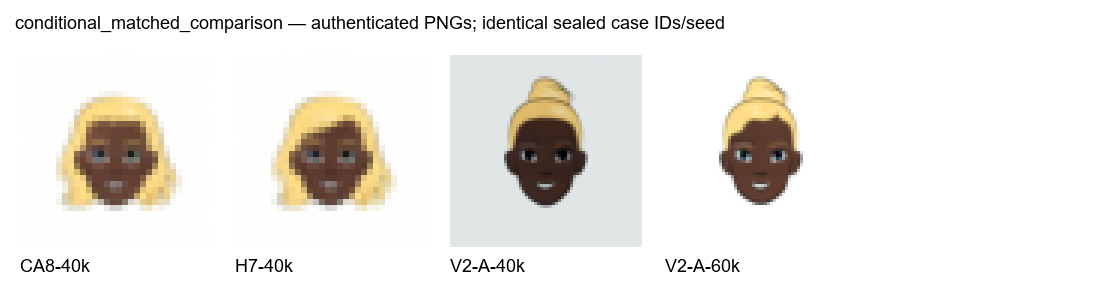
\includegraphics[width=.47\textwidth]{figures/conditional_matched_comparison.png}\hfill
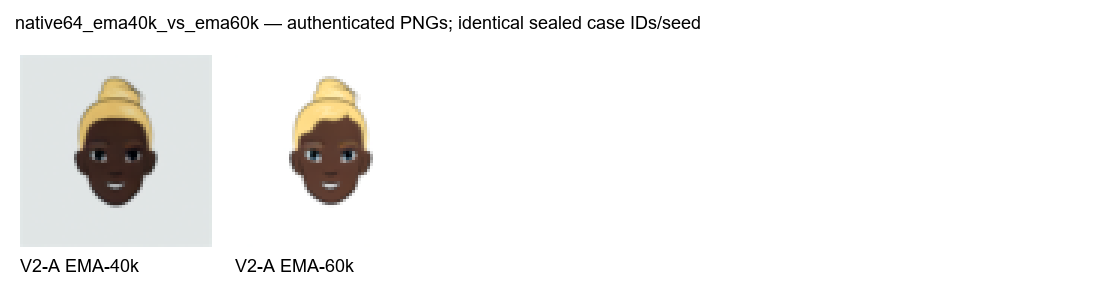
\includegraphics[width=.47\textwidth]{figures/native64_ema40k_vs_ema60k.png}
\caption{Authenticated same prompt/seed illustrative panels from the STEP~9B supplementary evidence. Left: conditional architecture comparison; right: V2-A conditional EMA-40k versus EMA-60k. They are not human ratings, independent tests, or visual proof of a single causal factor.}\label{fig:qualitative}
\end{figure*}
